\documentclass[a4paper, 11pt, twocolumn]{article}

\usepackage[utf8]{inputenc}

\usepackage[T1]{fontenc}

\usepackage[english]{babel}

\usepackage{graphicx}

 \usepackage{floatrow}
 
 \usepackage{caption}
 \usepackage{subcaption}

\usepackage[margin = 1in]{geometry}

\usepackage{float}

\usepackage[hidelinks]{hyperref}


\usepackage{url}

\usepackage{natbib}

%\usepackage[
%backend=biber,
%sorting=none
%]{biblatex}
\bibliographystyle{abbrvnat}
\setcitestyle{authoryear,open={(},close={)}}

\usepackage[most]{tcolorbox}

\usepackage{csquotes}

\usepackage{fancyhdr}


\usepackage{lipsum}

\usepackage{multicol}
%\addbibresource{references.bib}
\title{\Large Methods in Bioinformatics Project \\
\huge Review of "muscat detects subpopulation-specific state transitions from multi-sample multi-condition single-cell transcriptomics data"}


\author{Léopold Guyot}

\date{\today}

\begin{document}

\pagestyle{fancy}
\setlength{\headheight}{25.0117pt}
\fancyhead{}\fancyfoot{}
\fancyhead[L]{
\includegraphics[width = 0.2\textwidth]{img/LOGO_Universite__libre_bruxelles.png}}
\fancyhead[R]{Methods in Bioinformatics Project}
\fancyfoot[R]{\thepage}


\fancypagestyle{plainfooter}{
	\fancyhf{}  % Clear all headers and footers
	\fancyfoot[R]{\thepage}  % Page number in right footer
}

\onecolumn
\vspace*{-1.5cm}  % Adjust this value as needed
\begin{center}
	{\Large Methods in Bioinformatics Project}\\[1ex]
	{\huge Review of "muscat detects subpopulation-specific state transitions from multi-sample multi-condition single-cell transcriptomics data"}\\[2ex]
	{\large Léopold Guyot}\\[1ex]
	{\today}
\end{center}
 
\thispagestyle{plainfooter}
%\begin{tcolorbox}[breakable,colback=white,colframe=black,width=\dimexpr\textwidth+12mm\relax,enlarge left by=-6mm]

%\section*{Abstract}


%\end{tcolorbox}


\begin{multicols}{2}
\section{Introduction}

Single-cell RNA sequencing (scRNA-seq) has revolutionized transcriptomics by enabling gene expression profiling at the resolution of individual cells. Unlike bulk RNA-seq, which averages expression signals across thousands or millions of cells, scRNA-seq reveals cell-to-cell heterogeneity and uncovers distinct cellular subpopulations within complex tissues. This allows to provide crucial insights in biological mechanisms.

\textbf{FIND REAL EXAMPLE OF CELL HETERO IMPORTANCE}
In many biological and clinical contexts, it is essential to account for this cellular diversity. For instance, in immunology or oncology, the presence or absence of specific cell subtypes can have significant functional and diagnostic implications. scRNA-seq offers the granularity needed to capture such variation, making it indispensable for studies where subtle but biologically meaningful differences may be masked by population averages.

However, the analytical challenges of scRNA-seq data are considerable. The data are high-dimensional, sparse, and noisy due to dropout events and technical variability. Modeling gene expression at the single-cell level must account for these factors while also respecting the hierarchical structure of the data—cells nested within patients or experimental groups. Furthermore, the design of appropriate statistical models must balance sensitivity, specificity, and computational scalability.

To address these challenges, a variety of statistical models have been developed. The \texttt{scDD} method \citep{scdd} models gene expression as a mixture of distributions, enabling the detection of differential expression patterns beyond mean shifts, such as changes in modality or proportion. Mixed-effect models  incorporate both fixed effects (e.g., cell subpopulation) and random effects (e.g., patient) to account for intra-patient correlations and nested data structures.

The reviewed article \citep{muscat} proposes a pseudobulking approach, where cells are aggregated by the combination of cell subpopulation and patient. This results in a data structure resembling bulk RNA-seq, reducing noise. Once aggregated, well-established bulk RNA-seq methods such as \texttt{limma} \citep{limma}, \texttt{DESeq2} \citep{deseq2}, and \texttt{edgeR} \citep{edger} can be applied for differential expression analysis. This strategy leverages the robustness of bulk models while preserving important biological structure related to both cell type and biological replicates.


In this study, we aim to reproduce and evaluate the results presented in the reviewed paper, which investigated differential expression analysis strategies for scRNA-seq data. In that work, the authors used two real scRNA-seq datasets as the basis for simulating artificial datasets with known, controlled variations. These simulated datasets allowed for rigorous benchmarking of modeling approaches.

The original study compared different strategies: Single-cell methods including \texttt{scDD}, and mixed-effect models and aggregation-based methods, where cells were grouped by patient and subpopulation to produce pseudobulk profiles, then analysed using established bulk RNA-seq tools such as \texttt{limma}, \texttt{DESeq2}, and \texttt{edgeR}. 

\textbf{PREVIEW OF RESULTS}

\section{Methods}

This project was developed using the R programming language \citep{base} and leveraged packages from the Bioconductor repository \citep{bioc}.

\subsection{Datasets}

To evaluate the performance of pseudobulking methods, the datasets used had to satisfy specific criteria. In particular, each dataset needed to include multiple patients and several identifiable cell subpopulations. These datasets were then used to simulate new data that mimic the original distribution patterns.

\subsubsection{Kang et al. 2018}

The dataset from Kang et al. \citep{kang_multiplexed_2018} consists of single-cell RNA-sequencing profiles of peripheral blood mononuclear cells (PBMCs) collected from 8 human donors. It includes both unstimulated and interferon-$\beta$–stimulated cells.

The original droplet-based scRNA-seq data is publicly available via the Gene Expression Omnibus (GEO) under the accession \url{https://www.ncbi.nlm.nih.gov/geo/query/acc.cgi?acc=GSE96583}. It is also distributed in the \texttt{SingleCellExperiment} format \citep{sce} through the \texttt{ExperimentHub} package \citep{ExperimentHub}, using the accession code: \texttt{EH2259}.

\subsubsection{Mouse LPS}

The second dataset investigates transcriptomic changes in brain tissue from mice subjected to peripheral lipopolysaccharide (LPS) treatment. It includes samples from 4 vehicle-treated and 4 LPS-treated mice.

This dataset was originally published alongside the reviewed paper \citep{muscat}. It is accessible via ArrayExpress (accession: E-MTAB-8192) and can also be obtained from the \texttt{ExperimentHub} package \citep{ExperimentHub} with the accession code: \texttt{EH3297}.

\subsubsection{Guo et al. 2018}

Guo et al. \citep{guo_adult_2018} performed single-cell RNA sequencing on approximately 6,500 testicular cells from 3 healthy adult males, using the 10x Genomics Chromium platform.

This dataset was not included in the original benchmarking paper. It was added here as an independent dataset to assess the generalizability and robustness of the results obtained with other datasets. The aim is to evaluate whether similar conclusions can be drawn using a dataset with different biological context and origin.

The dataset is available through the \texttt{CTdata} R package \citep{CTdata}, and can be accessed using the \texttt{testis\_sce} function.


\subsection{Simulation Framework}

To systematically evaluate differential expression analysis methods, we developed a data-driven simulation framework based on a multi-sample, multi-subpopulation scRNA-seq reference dataset. This framework allows for modulation of key parameters, including the number of cells per subpopulation and sample, as well as the type and magnitude of differential expression patterns. Simulations are based on the negative binomial distribution, which is widely used to model scRNA-seq data. Subpopulation- and sample-specific parameters (means, dispersions, and library sizes) are estimated directly from the reference dataset. Simulated data is then generated by sampling from these empirical distributions, thereby capturing the structure and variability observed in real scRNA-seq data.

To introduce biologically meaningful variation, genes can be designated as subpopulation specific (differential across cell types), condition specific (differential expression between treatment conditions), or non-differential (uniform expression across all variables). 

The framework supports a diverse set of expression patterns based on the classification by Korthauer et al. \citep{korthauer2016statistical}:
\begin{itemize}
	\item \textbf{DE (Differential Expression)}: A change in the mean expression level of a gene between conditions, while the overall distribution shape remains unimodal and similar.
	\item \textbf{DP (Differential Proportion)}: A shift in the proportions of cells in low and high expression states between conditions, without a change in the expression values themselves.
	\item \textbf{DM (Differential Modality)}: A change in the modality of gene expression, such as shifting from a unimodal to a bimodal distribution, indicating that the underlying structure of expression changes.
	\item \textbf{DB (Differential Both)}: A combination of DP and DM, where both the proportions and the modality of expression states differ between conditions.
	\item \textbf{EE (Equally Expressed)}: No differences in expression or distribution between conditions or subpopulations; expression is consistent across all samples.
	\item \textbf{EP (Equal Proportion)}: Genes exhibit bimodal expression, but the proportions of cells in each expression state remain the same across conditions.
\end{itemize}

This classification enables simulation of complex and realistic gene expression scenarios, making the framework well-suited for benchmarking modelling methods across a variety of biologically plausible settings.

\subsection{Pseudobulk Approach}

To reduce the complexity of the data to be modeled, an aggregation approach can be applied. This involves summarizing the counts of cells belonging to a specific patient and a specific cell group (Fig. \ref{fig:pseudobulk}). Aggregation can be performed using different summary statistics, such as the sum or the mean. By applying this technique, we simplify the data and reduce the noise while preserving meaningful biological variation, specifically the variability between biological replicates and the variability between cell (sub)populations.
\begin{figure}[H]
	\centering
	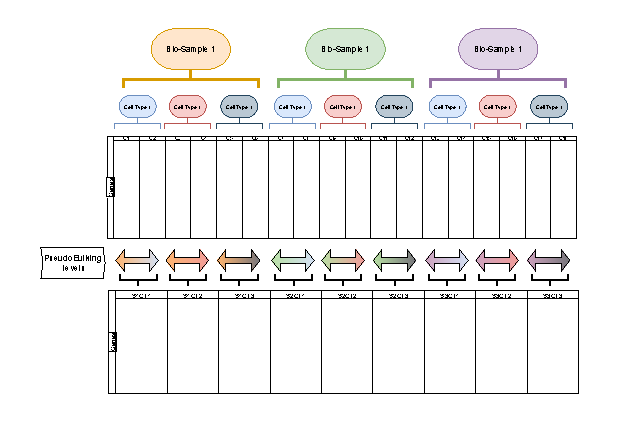
\includegraphics[width=1\columnwidth]{img/rnapseudobulk.drawio-1.pdf}
	\caption{{\footnotesize Scheme of the pseudobulk approach. The columns in the first table represent the individual cells. Several cells belonging to the same bio-sample and cell type are aggregated to give the second table in which each column represent the value for a particular bio-sample and cell type.}}
	\label{fig:pseudobulk}
\end{figure}

\subsection{Workflow}

\begin{figure}[H]
	\centering
	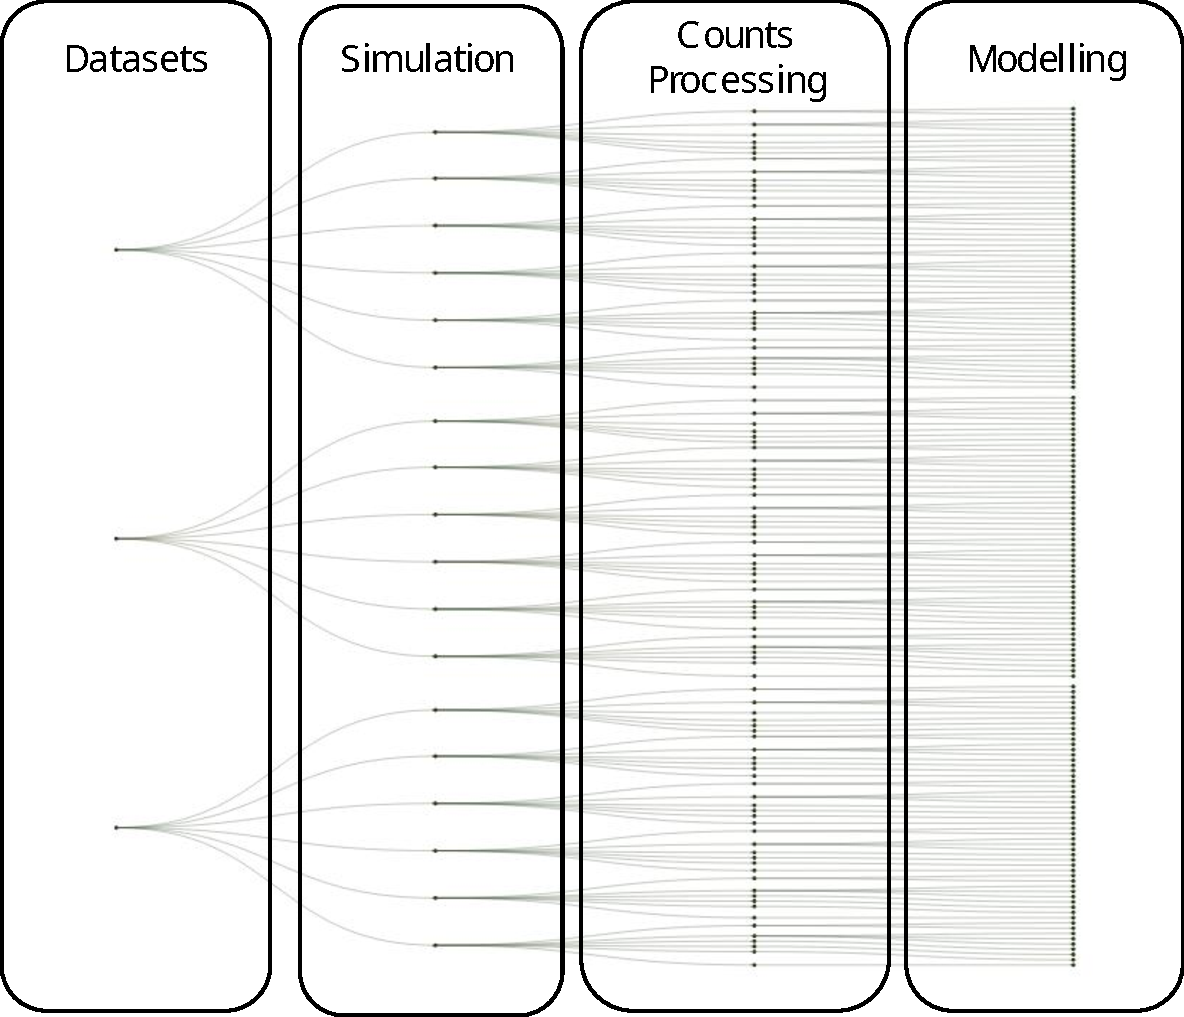
\includegraphics[width=0.8\columnwidth]{img/workflowCut.pdf}
	\caption{{\footnotesize Scheme of the workflow generated with \texttt{targets}. The first layer is the datasets retrieval and preprocessing. The second layer is the simulation of new datasets using different parameters. The third layer is the use of different processing method and aggregation techniques on counts. The fourth layer is the modelisation of the data.}}
	\label{fig:workflow}
\end{figure}

Given the complexity and number of steps involved in this workflow, we used the \texttt{targets} R package \citep{targets} to automate the entire process. Each step is applied to the results produced by all preceding steps, ensuring a consistent and reproducible pipeline. In total, the workflow comprises 291 steps and results in the generation of 144 models (Fig. \ref{fig:workflow}).

\subsubsection{Preprocessing}

Each dataset underwent a standardized preprocessing procedure. To ensure that only the intended variation was present, we retained a single experimental condition per dataset. Specifically, for the Kang et al. dataset, only the control cells were kept; for the mouse LPS dataset, only vehicle-treated cells were retained; and the testis dataset included only one experimental condition.

We filtered genes to retain those with more than one count in at least 10 cells. Similarly, we filtered cells to keep only those expressing at least 100 genes. Additionally, we retained only those clusters that consisted of at least 100 cells.

\subsubsection{Simulation}

The datasets were used to generate artificial data according to the simulation framework described earlier. We used functions provided by the \texttt{muscat} R package \citep{muscat} to facilitate the simulation process.

We simulated various scenarios using different parameter combinations. In the first set of simulations, each sample-subpopulation combination contained 400 cells. We considered four cases:
\begin{enumerate}
	\item 10\% of genes were altered in both proportion and modality.
	\item 10\% of genes were altered in mean expression.
	\item 10\% of genes were altered in modality.
	\item 10\% of genes were altered in the proportions of low and high expression-state components.
\end{enumerate}

Additionally, we conducted a series of simulations in which 10\% of the genes were altered in mean expression, varying the number of cells per sample-subpopulation combination (20, 100, and 400 cells).

\subsubsection{Processing Counts}

Each simulated dataset was processed using multiple count normalization methods. These included log-transformation, residuals, counts-per-million (CPM), and unprocessed raw counts. The transformations were performed using the \texttt{calculateCPM}, \texttt{normalizeCounts}, and \texttt{computeLibraryFactors} functions from the \texttt{scuttle} R package \citep{scatter}, as well as the \texttt{vst} function from the \texttt{sctransform} R package \citep{sctrans}.

\subsubsection{Pseudobulk}

We applied three different pseudobulk aggregation strategies: mean aggregation, sum aggregation, and no aggregation.

\subsubsection{Modelisation}

We employed a variety of models for differential analysis, using the formula \texttt{\textasciitilde{} patient + cell\_subpopulation}. For non-aggregated data, we applied mixed models and the \texttt{scDD} method. The mixed models were implemented using the \texttt{lmer} function from the \texttt{lme4} package \citep{lme4}, treating the patient effect as a random effect. The \texttt{scDD} method was implemented using the \texttt{scDD} package \citep{scdd}.

For aggregated (pseudobulk) data, we used established bulk RNA-seq modeling approaches, including \texttt{limma} \citep{limma}, \texttt{DESeq2} \citep{deseq2}, and \texttt{edgeR} \citep{edger}. The \texttt{limma} package was applied with either the \texttt{voom} or the \texttt{trend} method.

\subsubsection{Process Results}

The results were processed using the \texttt{iCOBRA} package \citep{icobra}. Differential expression tables were used to generate FDR–TPR curves at various adjusted \textit{p}-value thresholds (0.01, 0.05, 0.1, and 0.2) comparing the results between locally adjusted \textit{p}-value (at the cluster level) and globally adjusted \textit{p}-value. Additionally, UpSet plots were generated to visualize the intersections of detected gene sets across methods and ground truth. The runtime for each method, comprising both the aggregation and modeling steps, was recorded using the \texttt{targets} package \citep{targets}.
	
\section{Results}

\subsection{Effect of the Variation Type Introduced on Model Performance}

\subsubsection{Kang and LPS datasets}
To assess the impact of different expression variation types on method performance, we here show the simulation results based on the Kang dataset (Fig. \ref{fig:fdrtpr_prop_kang}) but the results obtained from the mouse LPS show equivalent results. These simulations introduced distinct categories of gene expression variation and allowed comparison of the true positive rate (TPR) and false discovery rate (FDR) across tested differential state methods.

\textbf{DB (Differential Both)} simulations showed consistently poor TPR across all tested methods. This is expected, as DB genes combine changes in both proportions and modality, presenting a particularly challenging scenario for current models. The inability to detect DB genes highlights the limitations of existing methods in capturing simultaneous changes in expression state prevalence and distribution structure.

In contrast, \textbf{DE (Differential Expression)} simulations demonstrated that pseudobulk methods outperformed both mixed models (MM) and scDD. Among the pseudobulk approaches, performance was generally strong, although \textit{limma-trend} applied to VST residuals showed a reduced TPR compared to other pseudobulk variants. scDD exhibited very low TPR; while locally adjusted p-values improved detection rates, this came at the cost of a notable increase in FDR.

\textbf{DM (Differential Modality)} simulation results were similar to those for DE, with aggregation-based methods again showing superior performance relative to MM and scDD. Notably, scDD, while still exhibiting low TPR, showed improved FDR control in this scenario compared to its performance on DE simulations.

\textbf{DP (Differential Proportion)} was the most challenging variation type among DE, DM, and DP. All methods exhibited a drop in TPR compared to DE and DM. In particular, \textit{limma-trend} using VST residuals failed to model the data effectively, with especially low TPR.

Overall, these results highlight the clear advantage of pseudobulk-based approaches across various expression variation types, particularly DE and DM. Mixed models and scDD lagged behind, especially in more complex or proportion-driven scenarios.
\subsubsection{Validation on an Independent Dataset: testis dataset} 
To assess the robustness of our observations, we additionally tested all methods with a newly added \textit{testis} dataset (Fig. \ref{fig:fdrtpr_prop_testis}). Globally, the results obtained on this dataset were consistent with those from the Kang and LPS datasets, reinforcing the validity of our conclusions. For most variation types, the relative performance of the methods remained similar. However, a notable deviation was observed for \textbf{DM (Differential Modality)} simulations: the \textit{limma-trend} method applied to VST residuals displayed a markedly elevated FDR, reaching up to 20\% false positives. This suggests that this approach may be unreliable for detecting modality-driven changes in certain biological contexts. Despite this exception, the overall agreement in trends between datasets increases our confidence in the comparative evaluation and the general applicability of the simulation framework.

\subsubsection{Impact of Count Processing Strategies}
Across all datasets and variation types, the choice of count processing strategy had minimal impact on model performance for most pseudobulk methods. However, one notable exception was observed for the \textit{limma-trend} method when applied to VST residuals. This count processing method consistently showed reduced TPR and, in some cases, increased FDR, particularly in the DE and DM scenarios.

\subsection{Effect of sample size on model performance}

We assess the impact of the number of cells per patient and subpopulation on model performance. The results were consistent across all datasets tested: Kang (Fig. \ref{fig:fdrtpr_size}), LPS (data not shown), and testis (Fig. \ref{fig:fdrtpr_testis}). This is confirming the generalizability of the observed trends.

As expected, model performance declined when the number of cells per patient/subpopulation decreased. This effect was evident in both true positive rate (TPR) and false discovery rate (FDR), with fewer cells leading to reduced sensitivity and less stable error control.

Importantly, the rate at which performance improved with increasing sample size was not uniform across methods. Notably, \textit{edgeR} and \textit{limma-trend} applied to mean-aggregated logcounts showed a steeper gain in performance between low (e.g., 20 cells) and moderate (e.g., 100 cells) cell counts compared to other methods. This suggests that these approaches are more sensitive to increases in data quantity and may be preferable in settings with moderate to high cell numbers per subpopulation. Other methods, while also benefiting from larger sample sizes, exhibited more gradual improvements, indicating differences in statistical efficiency or robustness to small sample regimes.

\end{multicols}

\begin{figure}[h]
	\centering
	\begin{subfigure}[t]{0.9\textwidth}
		\centering
		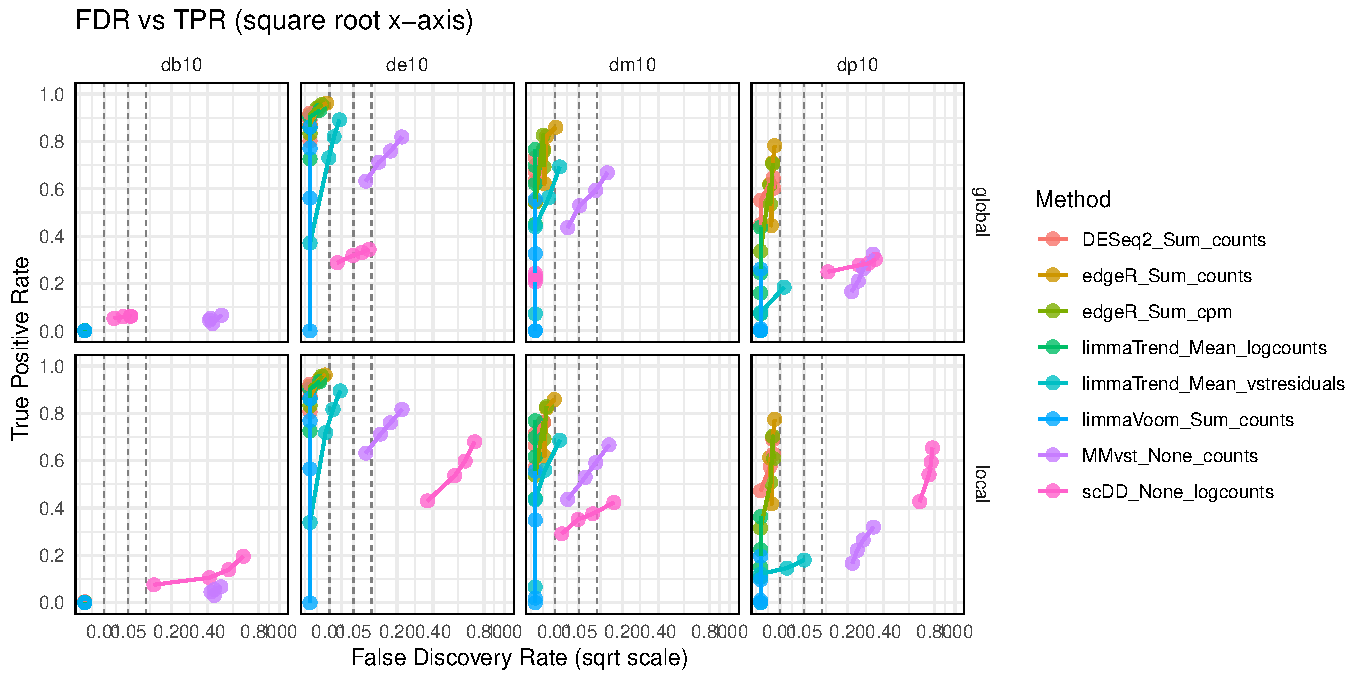
\includegraphics[width=\textwidth]{figs/fdrtpr_prop_method_Kang.pdf}
		\caption{FDR vs TPR by proportion}
		\label{fig:fdrtpr_prop_kang}
	\end{subfigure}
	
	\vspace{1em}
	
	\begin{subfigure}[t]{0.8\textwidth}
		\centering
		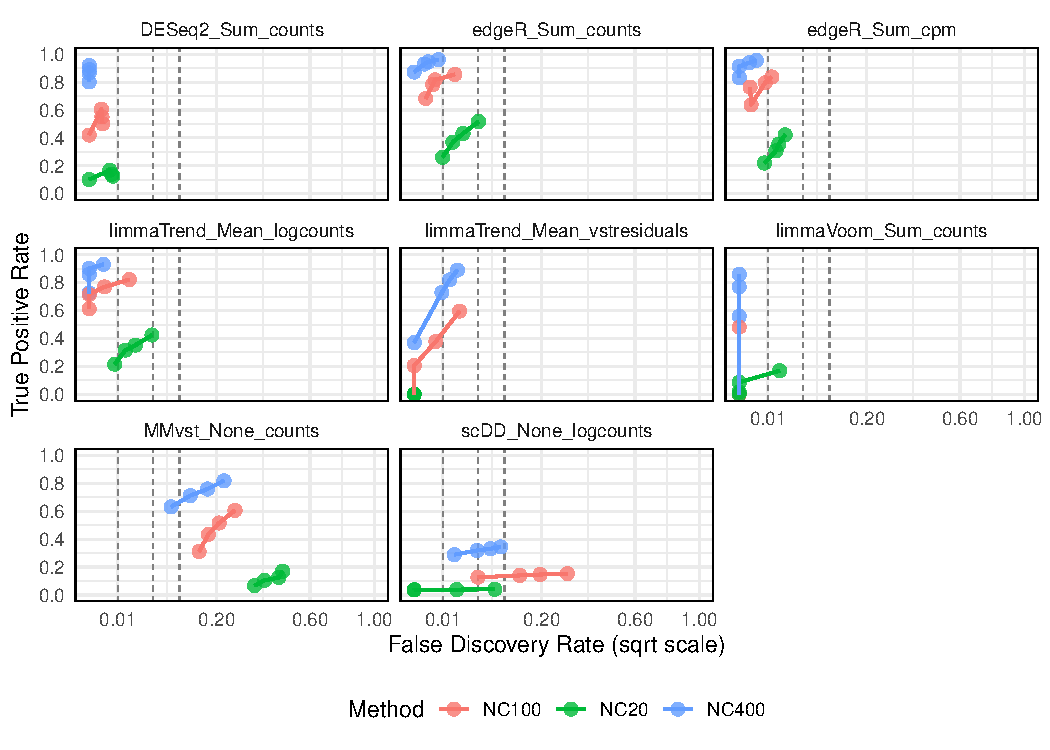
\includegraphics[width=\textwidth]{figs/fdrtpr_size_method_Kang.pdf}
		\caption{FDR vs TPR by sample size}
		\label{fig:fdrtpr_size}
	\end{subfigure}
	
	\caption{Comparison of FDR vs TPR under different experimental conditions: (a) varying proportions and (b) varying sample sizes.}
	\label{fig:fdrtpr_combined_kang}
\end{figure}


\begin{figure}[h]
	\centering
	\begin{subfigure}[t]{0.9\textwidth}
		\centering
		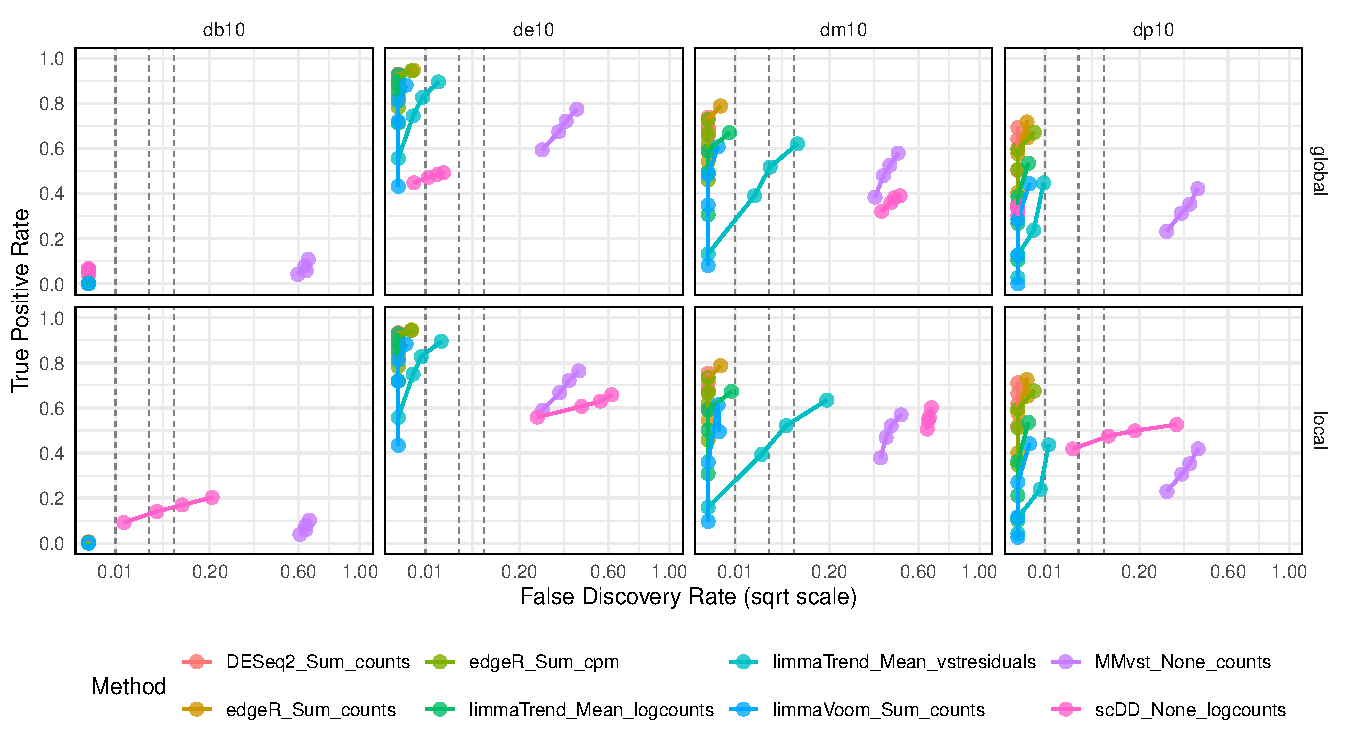
\includegraphics[width=\textwidth]{figs/fdrtpr_prop_method_Testis.pdf}
		\caption{FDR vs TPR by proportion}
		\label{fig:fdrtpr_prop_testis}
	\end{subfigure}
	
	\vspace{1em}
	
	\begin{subfigure}[t]{0.8\textwidth}
		\centering
		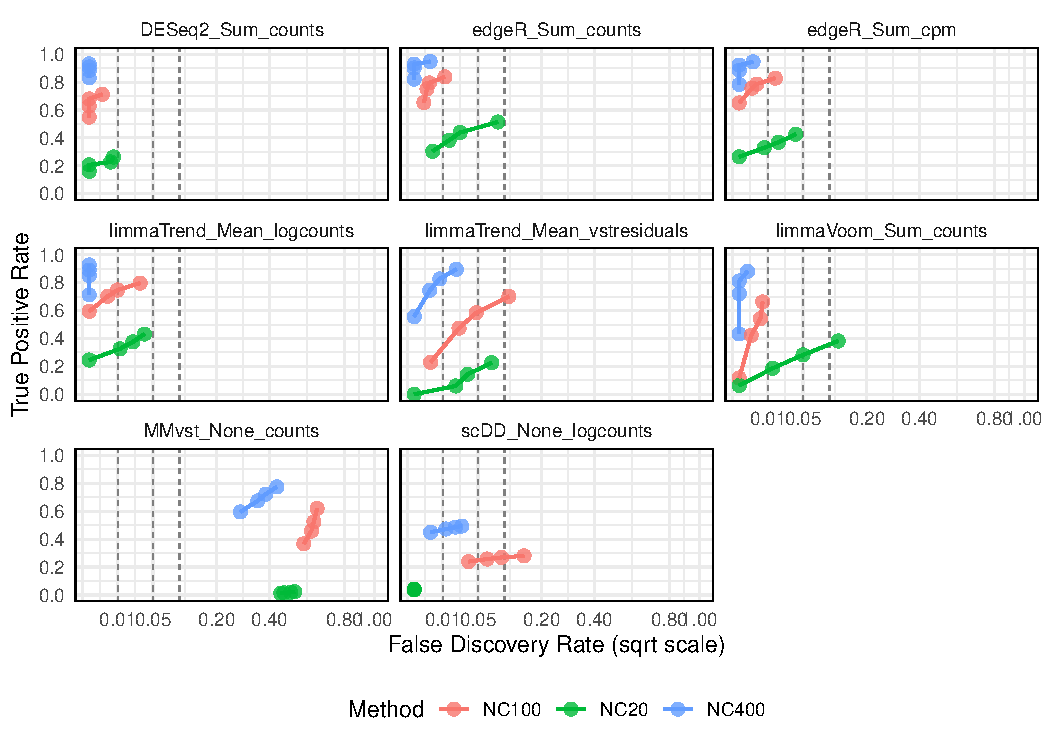
\includegraphics[width=\textwidth]{figs/fdrtpr_size_method_Testis.pdf}
		\caption{FDR vs TPR by sample size}
		\label{fig:fdrtpr_testis}
	\end{subfigure}
	
	\caption{Comparison of FDR vs TPR under different experimental conditions: (a) varying proportions and (b) varying sample sizes.}
	\label{fig:fdrtpr_combined_testis}
\end{figure}

\begin{multicols}{2}
	
\subsection{Runtime Analysis}

\begin{figure}[H]
	\centering
	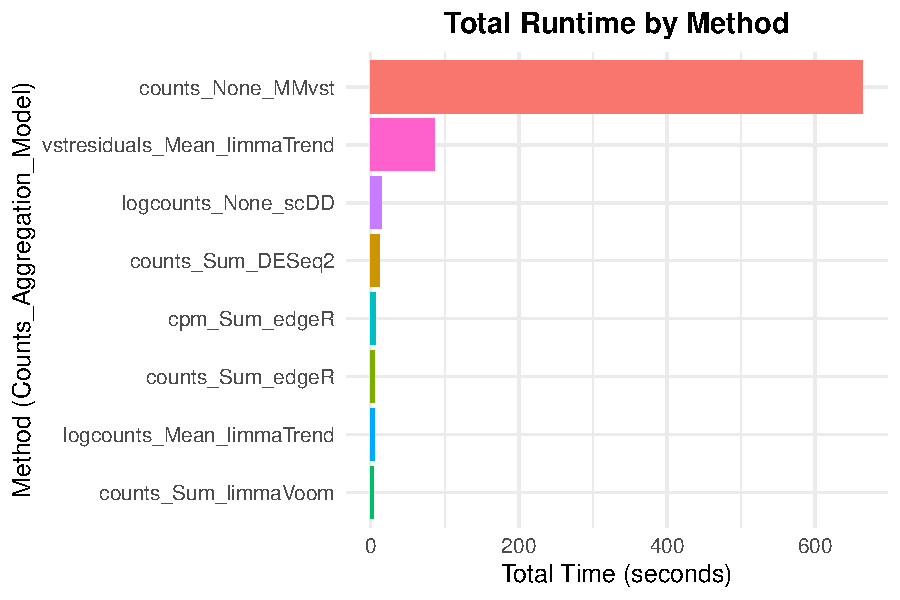
\includegraphics[width=1\columnwidth]{figs/plot_runtime_Kang.pdf}
	\caption{{\footnotesize Runtime analysis of the counts processing + aggregation and the modelisation. Time in seconds.}}
	\label{fig:runtime}
\end{figure}
\section{Discussion}

Difference between my setup: not replicates (too long)
Did not tested all the methods (AD)


Which issues did you identify, and which problems
did you encounter?
– What is different about your approach (and the
results you get) in comparison to the original
method? Why?
– What are advantages/disadvantage of each
method?
– 1 page
\section{Conclusion} 

\bibliography{references}
\end{multicols}
\end{document}
